\documentclass[notitlepage, twocolumn]{article}
\usepackage[left=0.6in, right=0.6in, top=1in, bottom=0.8in]{geometry}

\usepackage{titling}
\usepackage[compact]{titlesec}
\usepackage{lipsum}
\usepackage{graphicx}
\usepackage[labelfont=bf, labelsep=space]{caption}
\usepackage{subcaption}
\usepackage[noabbrev]{cleveref}
\usepackage{mwe}
\usepackage{sansmathfonts}
\usepackage{amsmath}
\usepackage{float}
\usepackage{fancyhdr}
\usepackage{cite}

\pagestyle{fancy}
\fancyhf{}
\fancyhead[LE,RO]{}
\fancyhead[RE,LO]{}
\fancyfoot[CE,CO]{}
\fancyfoot[LE,RO]{\thepage}
 
\renewcommand{\headrulewidth}{0.5pt}
\renewcommand{\footrulewidth}{0.5pt}

\renewcommand{\familydefault}{\sfdefault}

\titleformat*{\section}{\large\bfseries\uppercase}
\titleformat*{\subsection}{\bfseries}

\titlespacing*{\section}{0pt}{\baselineskip}{1pt}
\titlespacing*{\subsection}{0pt}{0.5\baselineskip}{1pt}

\renewcommand{\abstractname}{\vspace{-\baselineskip}} % Remove Abstract header

\newcommand\invisiblesection[1]{%
  \refstepcounter{section}%
  \addcontentsline{toc}{section}{\protect\numberline{\thesection}#1}%
  \sectionmark{#1}\phantom{}}

\DeclareCaptionFormat{myformat}{#1#2#3\hrulefill}
\DeclareCaptionLabelFormat{bold}{\textbf{(#2)}}
\captionsetup[figure]{format=myformat, subrefformat=bold}
\captionsetup[subfigure]{format=default}

\pretitle{\Huge}
\posttitle{\par\vskip 0.5em}
\preauthor{\bfseries}
\postauthor{}
\predate{\par\large\centering}
\postdate{\par}

\title{Unified variation discovery and genotyping from high-throughput sequencing data}

\newcommand*\samethanks[1][\value{footnote}]{\footnotemark[#1]}
\author{Daniel Cooke\thanks{Wellcome Trust Centre for Human Genetics, University of Oxford, Oxford, UK} \&
Gerton Lunter\samethanks}
\thanksmarkseries{arabic}
\date{}

\begin{document}

\maketitle
\thispagestyle{empty}

\begin{abstract}\textbf{
Haplotype-based variant callers, which consider physical linkage between variation sites, are currently the \emph{de facto} choice for germline variation discovery and genotyping. However, there is a notable lack of these tools beyond those aimed at detecting common germline variation in diploid human individuals. Here we show a flexible haplotype-based variant detection algorithm, Octopus, that incorporates a polymorphic Bayesian genotyping model capable of accurately characterising multiple variation sources. Octopus outperforms all existing germline, somatic, and \emph{de novo} mutation detection tools, offers the first general approach to probabilistic phasing directly from raw sequence data, and is readily extendible to atypical samples and new sequencing technology.
}\end{abstract}

\invisiblesection{Motivation}

Detection of genetic variation and genotyping from High-Throughput Sequencing (HTS) data is now commonplace in clinical diagnosis pipelines, and is rapidly replacing array based assays for phenotype association studies. The high resolution offered by sequencing empowers detection of rare variants not covered by genotype arrays; enables identification of small indels and larger structural variation; and in some instances can resolve haplotype structure with \emph{physical phasing} which provides important information for disease risk analysis and phylogenetic inference \cite{RN211}.

Over the past ten years, a number of variant detection algorithms which use HTS as input have been developed. Other than a handful of \emph{de novo} based assembly approaches \cite{RN148}, the majority of these methods are mapping based \cite{RN141, RN538, RN5}, which require raw sequencing reads first be aligned to a reference sequence using a read mapper. Na\"\i ve variant callers directly use read alignments provided from a read mapper by forming a pileup of read bases at each reference base, calls are then made at each position by comparing the proportion of reference and non-reference observations \cite{RN537}. These methods make the simplifying - but mistaken - assumption that the read alignments provided by the mapper against the reference are always correct. In contrast, haplotype-based methods only assume read mapping location is approximately correct and compare evidence for one or more read alignments under multiple hypothetical haplotypes. This is an improvement for two reasons. First, certain alignment-based errors, particularly evident around indel variants, are avoidable which reduces dependence on the read mapper. Second, the genotype posterior signal-to-noise ratio improves with haplotype length because the number of erroneous haplotypes increases exponentially while the number of true haplotypes remains constant. This makes haplotype based methods more powerful than equivalent positional methods \cite{RN166}.

All haplotype-based methods published to date all focus on germline variation in pooled sequencing studies, and employ similar genotyping models derived from population genetics to explain observed read data \cite{RN141, RN538, RN5}. Such models offer a poor approximation to data typically generated from other types of sequencing experiment, including tumour and bacterial sequencing. In other cases, valuable prior information, such as pedigree structure, is not fully utilised. This can result in a significant reduction in power to detect and classify real variation. Although na\"\i ve methods that implement more appropriate statistical models are often available, they often perform worse than poorly fitted haplotype-based tools. Researchers often resort implementing custom pipelines that involve post-hoc intersections of multiple caller outputs to obtain required inferences \cite{RN156, RN361, RN276, RN3, RN514, RN541, RN540}. This is especially prevalent for studies requiring somatic and \emph{de novo} mutation detection, which are often severely limited in ability to characterise all types of variation, potentially leading to misleading conclusions.

There are other important shortcomings in existing tools: First, sequencing errors are not adequately modelled; most methods \cite{RN538, RN141} assume uniform sequencing errors, but actual sequencing errors are often context-dependent \cite{RN149}, leading to falls calls; Second, read mapping qualities \cite{RN138} are often inadequately modelled, which can reduce specificity; Third, haplotype lengths are usually short as the number of possible haplotypes increases exponentially with the number of candidate variants, this is especially problematic in highly polymorphic regions, which can induce boundary artefacts resulting in false calls, or the region being skipped entirely.

Finally, phase information is becoming increasingly valuable to resolve population haplotype structure and infer functional effects of co-mutations \cite{RN211}. Obtaining variant phase directly from raw sequence data is challenging because phase and genotype inference is confounded as there is uncertainty in variant and genotype calls in addition to uncertainty in any particular haplotype structure. Although some existing methods implement non-probabilistic physical phasing algorithms \cite{RN538}, these approaches cannot resolve regions with weak read support or capture biologically meaningful information available in the genotype model, such as inheritance patterns. Therefore, existing methods are usually only able to offer phased calls over regions smaller than one read length with unambiguous strong read support \cite{RN538}.

We sought to address these issues by designing a method that treats haplotype generation, read error modelling, genotype inference, and phasing independently. This allows us to apply the most appropriate statistical model at each stage, whilst taking advantage of common haplotype generation machinery. We designed a statistical phasing algorithm based off genotype posterior distributions that is able to achieve far greater phase lengths than existing tools, sometimes well beyond one read length. Our algorithm is implemented in a C++14 application, \textit{Octopus}, which is freely available to all.

\section*{Results}

\subsection*{Haplotype generation}

The performance of haplotype-based methods is bounded by the ability to propose true haplotype sequences. The probability a true haplotype is observed in the read data is conditional on the underlying sample genotypes; some haplotypes may inherently have low observation probability (e.g. in tumour samples). It is therefore crucial to be able to achieve high sensitivity at this stage whilst being conscious of the increased computational burden of proposing many wrong haplotypes.

Haplotype construction begins by extracting putative alleles directly from the read alignments, although this can be augmented by external sources. Our algorithm distinguishes alleles from haplotypes: alleles are atomic mutation events whilst haplotypes are ordered sets of non-overlapping alleles. By default two methods are used for read-based allele generation: (i) variants supported directly from read alignments; (ii) variants identified via local re-assembly. The former method is usually more robust as it is only dependent on the alignment routine used by the mapper. Whilst the latter is able to resolve complex variation which may not be present in the read alignments due to inadequate read length. The main drawback of the latter approach is that it is highly sensitive to kmer size used and the genomic region selected for assembly, which can result in high quality variants being missed. By integrating both approaches, our algorithm is able to achieve higher sensitivity than other approaches which use one or the other \cite{RN141, RN538}.

Haplotypes are exhaustively constructed from all viable allele combinations. This differs from other approaches which construct haplotypes directly. The advantage of our approach is that haplotypes not directly supported by any particular read alignment can be proposed which enables arbitrary extension of existing haplotypes, enabling posterior based phasing beyond a single read length. The main limitation is that the number of haplotypes is exponential in the number of alleles, which restricts the length of candidate haplotypes (windowing). We have solved this issue by developing a graph-based data-structure, dubbed a 'haplotype-tree'. Nodes in the tree are alleles, and branches are unique haplotypes. Branches can be readily extended and pruned, accelerated by a hash-table lookup. This enables haplotypes with low posterior support to be removed from the tree before proliferation. This procedure can be repeated to obtain arbitrary long haplotypes whilst keeping the number of haplotypes under consideration roughly linear.

\subsection*{Genotype inference and variant calling}

The algorithm proceeds by calculating likelihoods for each read conditional on each haplotype using a Hidden Markov Model (HMM). Base mismatch and indel emission distributions are dependent on surrounding sequence context and sequencing technology, the former is derived from base quality scores. Error penalties occurring outside the current active region are deducted by following the Viterbi path. It may then be necessary to eliminate some haplotypes using likelihood based statistics to produce a final set of haplotypes.

\begin{figure*}[ht]
    \centering
    \begin{subfigure}[b]{0.3\textwidth}
        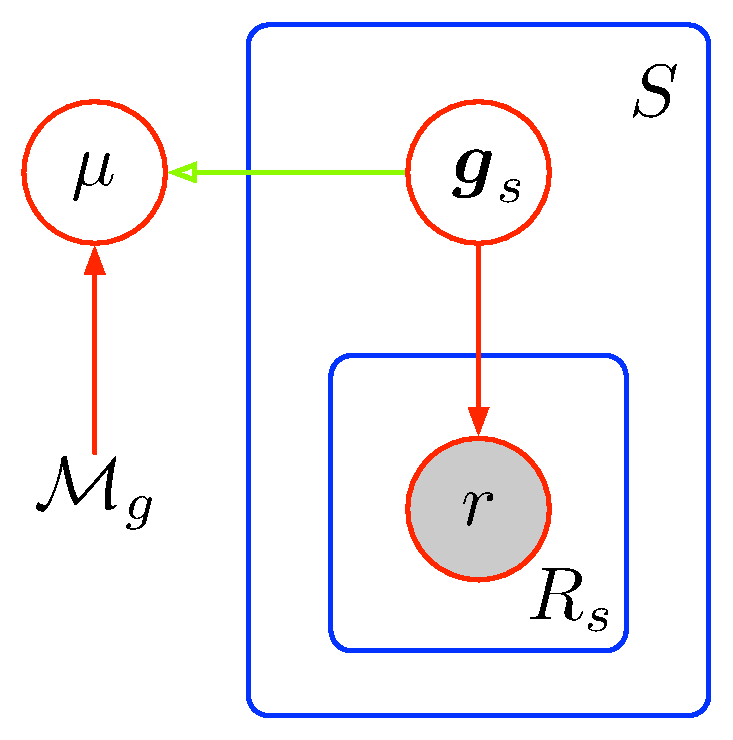
\includegraphics[width=\textwidth]{figures/population_model}
        \caption{}
        \label{fig:pop}
    \end{subfigure}
    \hfill
    \begin{subfigure}[b]{0.3\textwidth}
        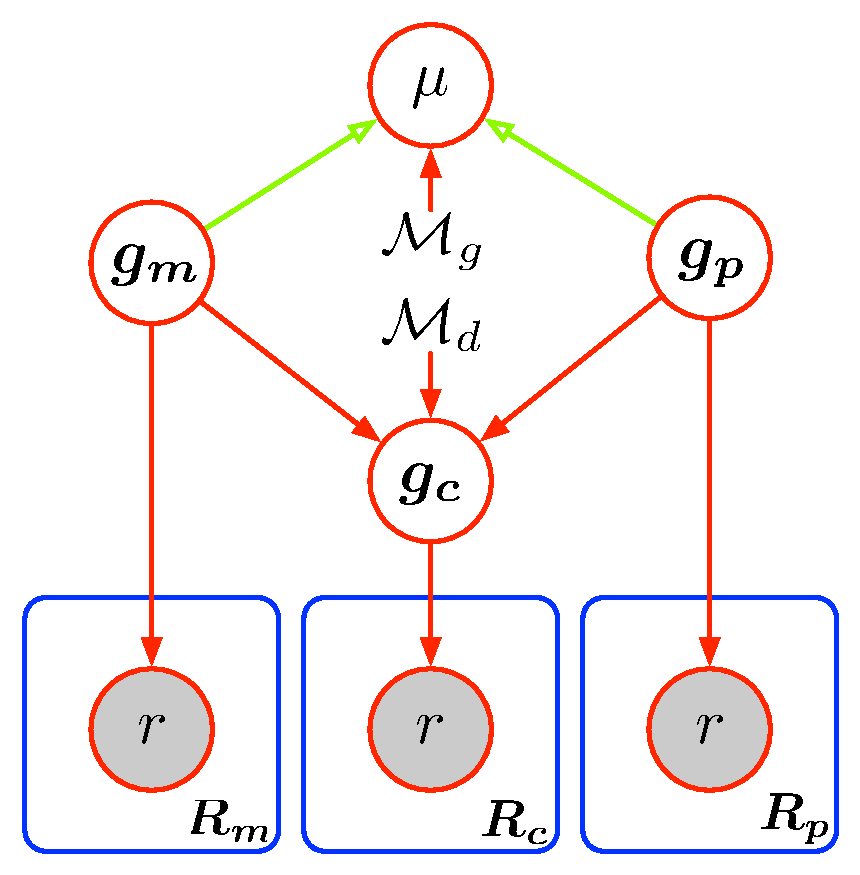
\includegraphics[width=\textwidth]{figures/trio_model}
        \caption{}
        \label{fig:trio}
    \end{subfigure}
    \hfill
    \begin{subfigure}[b]{0.3\textwidth}
        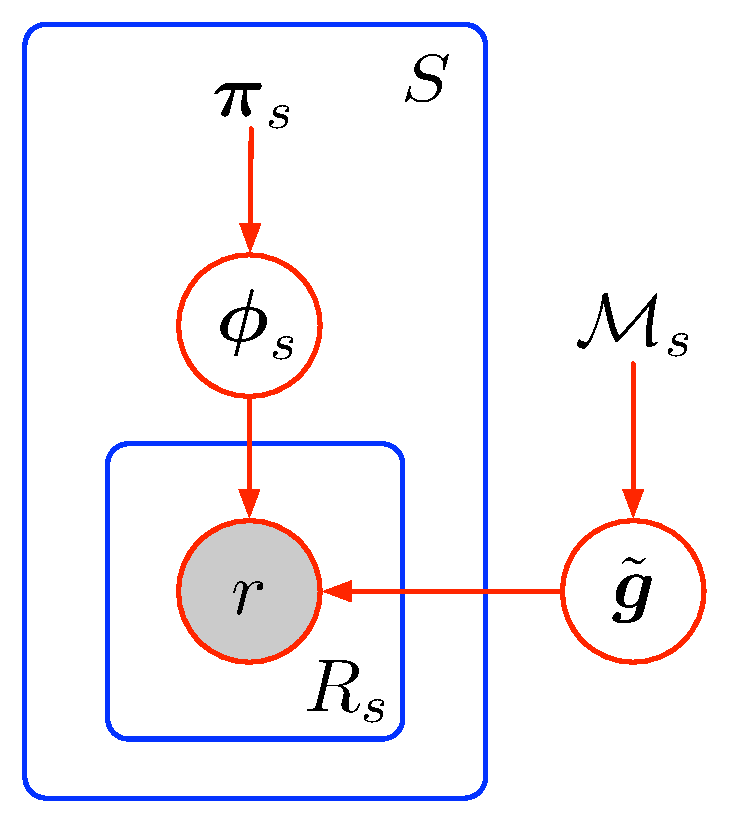
\includegraphics[width=\textwidth]{figures/cancer_model}
        \caption{}
        \label{fig:cancer}
    \end{subfigure}
    \caption{Genotype models shown in graph notation: \protect\subref{fig:pop} population, \protect\subref{fig:trio} trio, and \protect\subref{fig:cancer} tumour. Symbols insides circles are latent variables, observed variables are shaded. Symbols inside boxes are repeated. Symbols not inside a circle are parameters or models. Arrows define conditional relationships, red for stochastic and green for deterministic.}
    \label{fig:models}
\end{figure*}

The next step of the algorithm is to calculate posterior probability distributions for all  Bayesian genotype model latent variables (\textbf{Figure \ref{fig:models}}), which are used by \emph{calling models} to make variant, genotype calls, and any other sample-type specific inferences.

The population model is applicable to a set of samples of known ploidy and unknown pedigree. Variations of this model are implemented by most existing methods \cite{RN538, RN141, RN5, RN537}. For the case of a single sample the model simplifies to:

\begin{equation*}
    p(\boldsymbol{g} | \boldsymbol{R}, \mathcal{M}_{g}) \propto p(\boldsymbol{g} | \mathcal{M}_{g}) \prod_{r \in \boldsymbol{R}} \frac{1}{|\boldsymbol{g}|} \sum_{i = 1}^{|\boldsymbol{g}|} p(r | \boldsymbol{g}_i)
\end{equation*}

where $p(\boldsymbol{g} | \mathcal{M}_{g})$ is a germline prior model. For more than one sample exact inference is usually intractable and approximations are required. Genotype likelihoods are first computed under a simpler model using Expectation Maximisation \cite{RN5}, and then high likelihood genotype combinations are used to compute posterior probabilities under the Bayesian model.

The trio model is appropriate for parent-offspring trios as the genetic inheritance of genetic information from parent to child can be explicitly modelled. The parent-child relationship is stochastic as there is uncertainty in the inherited haplotype and because of \emph{de novo} mutations during meiosis. Recombination is not considered. Parental genotypes are assumed to share information as in the population model. This model can be computed exactly in most cases.

The tumour model is intended to model populations of somatically mutated heterogeneous tumour cell samples from the same individual. In contrast with the other models, the genotype latent variable in this model is augmented with an additional haplotype to capture somatically mutated tumour genotypes. Although more than one unique \emph{somatic haplotypes} are possible, such observations are rare over typically considered region lengths (up to a few kb) \cite{RN86}. Also unlike the other models, the tumour model does not assume equal genotype mixture weights to reflect the possibility of low-frequency alleles observations due to local copy-number changes and tumour cell impurity caused by heterogeneous sub-clonal sampling and normal contamination. To explicitly model sub-clonal cell populations, each sample has independent mixture priors, which also allows implicit modelling of a normal sample. Approximate posterior probability distributions are assigned to genotypes and sample mixtures using a Variational Bayes algorithm.

Variant calls are made by marginalising over the relevant posterior probability distributions assigned by the calling model. Posterior inferences may also include a Bayesian model comparison to reduce false positive calls due to poor model fit. In particular, somatic mutation calls are only made if the \emph{evidence} for the tumour model is significantly higher than the evidence for the population model (with a single sample). For germline calling, evidence comparison with a incremented ploidy model may be used to detect false positive variant calls caused by mapping errors. For each allele, unphased genotype probabilities (in allele space) are calculated by marginalising over full genotype posterior distributions (in haplotype space).

\subsection*{Statistical phasing}

The genotype posterior probability distributions computed in the last step are used to compute physical phasing of called variant sites. No read data is required as all information available from the read data as well as any prior information is contained in the posterior distributions.

\begin{figure}[ht]
\centering
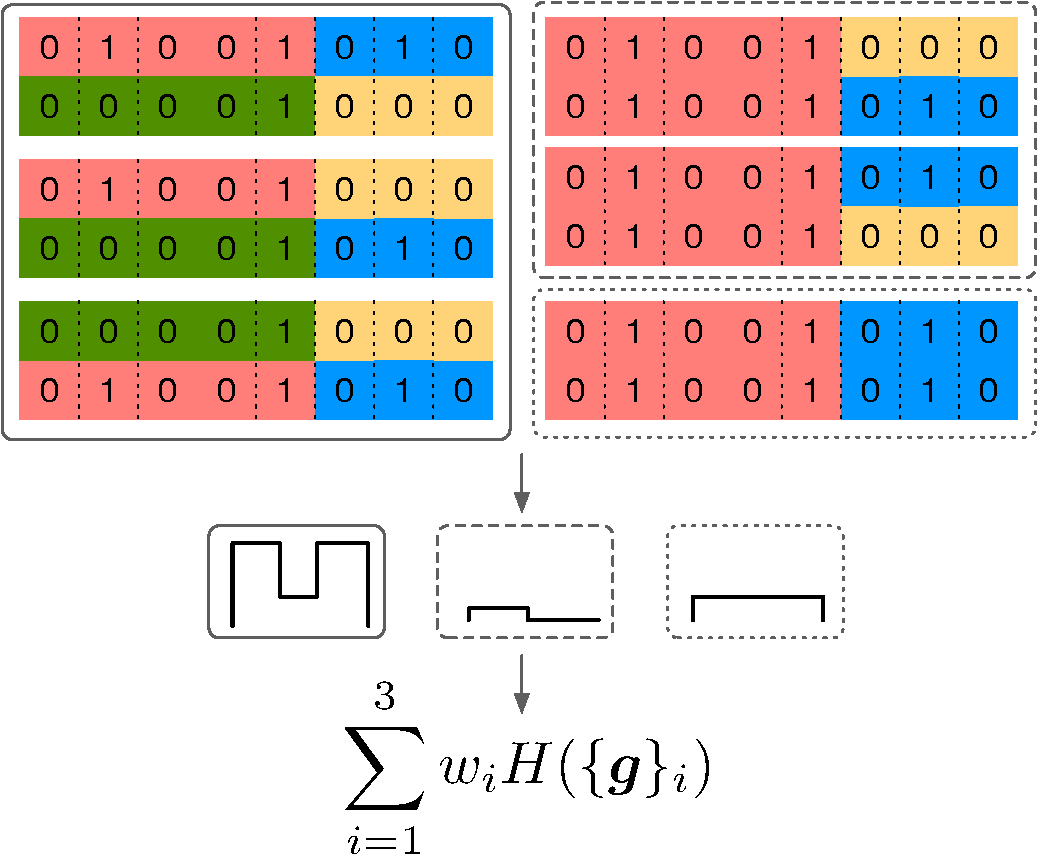
\includegraphics[width=0.5\textwidth]{figures/phasing}
\caption{Posterior based variant phasing with phase complement sets: Genotypes are partitioned into phase complement sets which are used to calculate a phase score, the weighted entropy of each phase complement set. The painted haplotypes show one possible local allele boundary.}
\label{fig:phasing}
\vspace{-1.5em}
\end{figure}

Samples are phased independently. First, all possible genotypes are partitioned into  'phase complement' sets (genotypes that share the same alleles at every site), there is only one such partitioning (\textbf{Figure \ref{fig:phasing}}). A phase score is defined as the weighted entropies of each normalised phase complement set, with respect to the genotypes present in each phase complement set. Low phase scores indicate less ambiguous phasing. The phasing algorithm finds the smallest set of genomic subregions such that each subregion has a phase score below a given value. 

\subsection*{Germline variants from WGS}

Although germline variant calling is a mature field, recent benchmark studies have shown there is still surprisingly low concordance between callers, and performance is highly dependent on the mapper used \cite{RN162, RN163}. To assess the performance of our algorithm on whole-genome data we used variants from the well studied 1000G sample NA12878, using the gold-standard high confidence calls provided by the Genome in a Bottle (GIAB) consortium \cite{RN153} as a benchmark. We made nine call-sets for each caller, one for each coverage-mapper combination (mappers: BWA-mem \cite{RN539}, Bowtie2 \cite{RN164}, and Novoalign). Calls were compared using RTG-tools \cite{RN169} which is more accurate than na\"\i ve intersection methods as calls are compared at a haplotype level. We compared our algorithm to four widely used tools, GATK HaplotypeCaller \cite{RN141}, Freebayes \cite{RN538}, Platypus \cite{RN5}, and Samtools \cite{RN537}. 

\begin{figure}[ht]
\centering
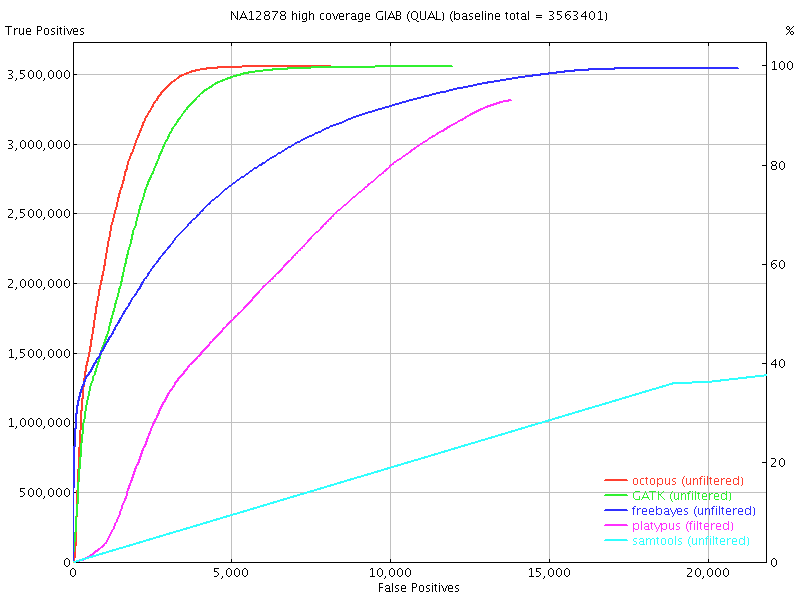
\includegraphics[width=0.5\textwidth]{figures/giab-benchmark}
\caption{ROC curves comparing variant callers on GIAB high confidence calls.}
\label{fig:giab}
\vspace{-1.5em}
\end{figure}

\subsection*{Germline variants from exome-capture}

Many clinical pipelines use exome-capture sequencing to detect disease risk variants. While in principal exome variant calling is easier than whole genome calling, due to differences in library preparation and sequencing depth, there are subtle artefacts present in exome data not in whole genome sequence data. We sought to evaluate the performance of our algorithm on clinical exome-capture sequence data. We compared our method to other tools by callings variants in the ICR 142 validation series data \cite{RN154} which includes positive and negative Sanger validation sites for a number of exome samples.

\begin{table}[ht]
\centering
\caption{ICR142 series summary}
\begin{tabular}{lcccc}
\hline
\multicolumn{5}{r}{ICR142 sites} \\
\cline{2-5} & TP & FP & TN & FN \\
\hline
Octopus & 0 & 0 & 0 & 0 \\
GATK HC & 0 & 0 & 0 & 0 \\
Freebayes & 0 & 0 & 0 & 0 \\
Platypus & 0 & 0 & 0 & 0 \\
Samtools & 0 & 0 & 0 & 0 \\
\hline
\end{tabular}
\end{table}

\subsection*{Somatic mutations in paired tumour-normal samples}

Cancer is a genetic disease caused by mutations that lead to uncontrollable cell division. Different cancers are driven by different sets of mutations to different gene pathways. A crucial step to understanding cancer; how to provide new diagnostics and therapies, is to accurately be able to genotype somatic mutations in tumours. Cancer genomes are often highly mutated, containing structural variation that alters local copy number. Cells from the same tumour form pockets of genetically heterogenous clones, and there is little guarantee of clone representation in the final sequencing library. All this makes the detection of somatic mutations challenging, particularly if the inaccurate assumptions are made when modelling the observed data. In particular, germline ploidy assumptions are likely to lead to low sensitivity to low allelic frequency somatic mutations. A number of bespoke somatic mutation detection tools have been developed in an attempt to address these issues \cite{RN142, RN146, RN150, RN143, RN145}. While these algorithms provide more appropriate models than advanced germline variant callers, none, other than a recent update to MuTect (Mutect2) are haplotype-based.

To demonstrate the accuracy of our method at calling somatic mutations in tumour-normal paired cancer samples, we compared the sensitivity and specificity of our method to popular somatic callers MuTect, Mutect2, SomaticSniper, Radia, Strelka, and VarScan2.

\subsection*{Somatic mutations in tumour only samples}

Reliable paired normal tissue samples are not always available when studying tumours from cancer patients, either because of restrictions present in a clinical setting, or because samples are archival. Most somatic mutation callers require a paired normal sample \cite{RN142, RN146, RN150, RN143, RN145}, although a recent tool was made available to specifically to deal analyse tumour only samples \cite{RN161}. We looked to test the robustness of our algorithm by running the previous samples without the paired normal samples, and compared these calls to our previous calls, and to those made by SomVarIUS.

\subsection*{\emph{De novo} mutations in parent-offspring trios}

Random germline \emph{de novo} mutations resulting from imperfections in the DNA replication process during meiosis provide the necessary genetic variation for evolution. They are also known to be causative of several Mendelian and polygenic diseases \cite{RN157, RN160, RN159}. Large scale characterisation of \emph{de novo} mutations in population studies reveals important insights into population structure and demographic history \cite{RN158}. The fidelity of the DNA replication process means the number of \emph{de novo} mutations expected per genome duplication event is small, usually less than 100 mutations per duplication in humans \cite{RN6}.

\subsection*{Bacterial calling using HTS data}

HTS is rapidly replacing culture based assays to diagnose infectious diseases in the clinic. Its potential to detect and identify strains means that can be used to establish drug-susceptibility profiles that potentially offers patients faster, more accurate diagnosis, and hence targeted treatment. This is especially important when patients present with multiple drug-resistant bacterium such a Mycobacterium Tuberculosis; a specific early diagnosis can result in life-saving treatment.

Some bacteria have high mutation rates resulting in high degrees of heterogeneity in a sample; with small fraction of cells containing a mutation. In addition, patients may be infected with multiple strains of the same species resulting in pseudo-poly-ploidy genotypes. These conditions render many germline variant calling tools inappropriate and underpowered \cite{RN165}.

\subsection*{Genotyping HLA loci}

\subsection*{Detection of structural variation}

\section*{Discussion}

As the use of high-throughput sequencing technology expands to new types of organisms, cells, and library preparation techniques, we will need new algorithms to accurately re-assemble the underlying genetic material of these assays. Current approaches are either too rigid or too simple, which limits the potential of the data we generate. We introduce a method that is able to achieve class-leading performance for multiple data types using a powerful core Bayesian framework, and is readily extendible to new types of sample. We hope researchers with niche samples that are unsatisfied with existing tools will be interested in our method.

Single-cell methods will soon enable us to accurately sequence the genomes of individual cells, potentially revolutionising the way we characterise germline and tumour genomes. As our understanding of molecular biology improves, we will be able to devise better statistical models to explain single cell data. Octopus offers an exciting opportunity to implement these models to uncover new insights into genetic variation within individuals.

\bibliographystyle{plos2009}
\bibliography{main}

\section*{Online methods}

\subsection*{Haplotype likelihood filtering}

For efficiency reasons, it may sometimes be necessary to reduce the haplotype set before genotype inference. While there is no silver bullet solution, we have found likelihood based approaches are most effective.

\subsection*{Coalescent priors}

The default germline prior model, $\mathcal{M}_{g}$, is a coalescent based model, $\mathcal{M}_{coal}$, is used in all models. The somatic prior model, $\mathcal{M}_s$, is also partially defined in terms of $\mathcal{M}_{coal}$, for the germline component of the augmented genotype. This model has two heterozygosity parameters $\theta_{1}$ and $\theta_{2}$ for SNP and indel variants respectively. Indel heterozygosities are known to vary considerably depending on sequence context, we therefore define $\theta_{2} = \lambda(s) \theta'_{2}$ where $\lambda(s)$ is a function of the surrounding sequence context $s$ and $\theta'_{2}$ is the baseline indel heterozygosity. Given a set of haplotypes, $H$, which could be a genotype, we calculate the union of segregating snp and indel sites, $k_{1}$ and $k_{2}$, between $H$ and the reference haplotype. Then $p(H | \mathcal{M}_{coal})$ is:

\begin{equation*}
    p(k_{1}, k_{2} |  \theta_{1}, \theta_{2}) = \binom{\theta_{1}}{\theta_{1} + \theta_{2}}^{k_1} \binom{\theta_{2}}{\theta_{1} + \theta_{2}}^{k_{2}} \binom{k_{1} + k_{2}}{k_{1}} p_{\theta_{1} + \theta_{2}} (k_{1} + k_{2})
\end{equation*}

Where $p_\theta(S = k)\sum_{i=2}^n (-1)^i \binom{n - 1}{i - 1} \binom{i - 1}{\theta + i - 1} \binom{\theta}{\theta + i - 1}^k$.

\subsection*{Population model approximation}

\subsection*{Trio model priors}

The key component in the trio model is the conditional offspring genotype prior probability $p(\boldsymbol{g_c} | \boldsymbol{g_m}, \boldsymbol{g_p}, \mathcal{M}_{denovo})$. 

\subsection*{Estimation of somatic allele frequency}

\subsection*{Marginalisation of genotype posteriors}

\end{document}